
\documentclass[border=12pt, multi, tikz]{standalone}
\usepackage{import}
\subimport{plotneuralnet/layers/}{init}
\usetikzlibrary{positioning}
\usetikzlibrary{3d}
\usetikzlibrary{calc}

\def\ConvColor{rgb:yellow,5;red,2.5;white,5}
\def\ConvReluColor{rgb:yellow,5;red,5;white,5}
\def\PoolColor{rgb:red,1;black,0.3}
\def\UnpoolColor{rgb:blue,2;green,1;black,0.3}
\def\FcColor{rgb:blue,5;red,2.5;white,5}
\def\FcReluColor{rgb:blue,5;red,5;white,4}
\def\SoftmaxColor{rgb:magenta,5;black,7}   
\def\SumColor{rgb:blue,5;green,15}

\newcommand{\copymidarrow}{\tikz \draw[-Stealth,line width=0.8mm,draw={rgb:blue,4;red,1;green,1;black,3}] (-0.3,0) -- ++(0.3,0);}

\begin{document}
\begin{tikzpicture}
\tikzstyle{connection}=[ultra thick,every node/.style={sloped,allow upside down},draw=\edgecolor,opacity=0.7]
\tikzstyle{copyconnection}=[ultra thick,every node/.style={sloped,allow upside down},draw={rgb:blue,4;red,1;green,1;black,3},opacity=0.7]

\node[canvas is zy plane at x=0] (scan) at (-4,0,0) {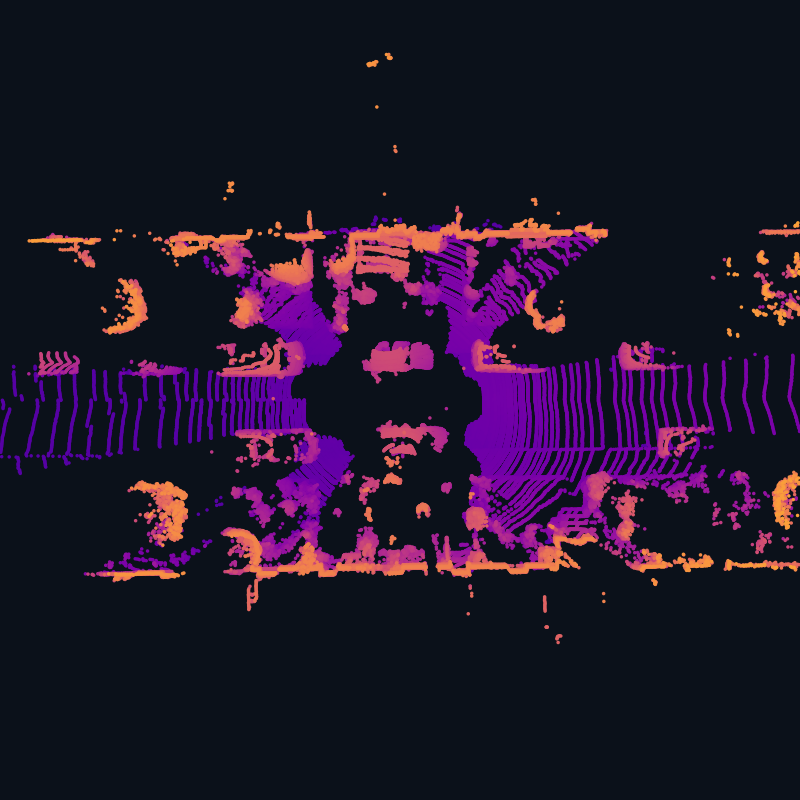
\includegraphics[width=9cm,height=9cm]{scan_input.png}};

\pic[shift={(0,0,0)}] at (0,0,0) 
    {Box={
        name=stem,
        caption=Stem\\10 cm,
        xlabel={{32, }},
        zlabel=,
        fill=\ConvColor,
        height=40,
        width=2.0,
        depth=40
        }
    };

\pic[shift={ (0,0,0) }] at (stem-east) 
    {Box={
        name=down1,
        caption= ,
        fill=\PoolColor,
        opacity=0.5,
        height=34,
        width=1,
        depth=34
        }
    };

\pic[shift={ (1.1,0,0) }] at (down1-east) 
    {RightBandedBox={
        name=enc1,
        caption=Enc 1\\20 cm,
        xlabel={{ , 32 }},
        zlabel=,
        fill=\ConvColor,
        bandfill=\ConvReluColor,
        height=32,
        width={ 2.0 , 2.0 },
        depth=32
        }
    };

\draw [connection]  (down1-east)    -- node {\midarrow} (enc1-west);

\pic[shift={ (0,0,0) }] at (enc1-east) 
    {Box={
        name=down2,
        caption= ,
        fill=\PoolColor,
        opacity=0.5,
        height=26,
        width=1,
        depth=26
        }
    };

\pic[shift={ (1.1,0,0) }] at (down2-east) 
    {RightBandedBox={
        name=enc2,
        caption=Enc 2\\40 cm,
        xlabel={{ , 64 }},
        zlabel=,
        fill=\ConvColor,
        bandfill=\ConvReluColor,
        height=25,
        width={ 2.8 , 2.8 },
        depth=25
        }
    };

\draw [connection]  (down2-east)    -- node {\midarrow} (enc2-west);

\pic[shift={ (0,0,0) }] at (enc2-east) 
    {Box={
        name=down3,
        caption= ,
        fill=\PoolColor,
        opacity=0.5,
        height=19,
        width=1,
        depth=19
        }
    };

\pic[shift={ (1.1,0,0) }] at (down3-east) 
    {RightBandedBox={
        name=enc3,
        caption=Enc 3\\80 cm,
        xlabel={{ , 128 }},
        zlabel=,
        fill=\ConvColor,
        bandfill=\ConvReluColor,
        height=17,
        width={ 3.8 , 3.8 },
        depth=17
        }
    };

\draw [connection]  (down3-east)    -- node {\midarrow} (enc3-west);

\pic[shift={ (0,0,0) }] at (enc3-east) 
    {Box={
        name=down4,
        caption= ,
        fill=\PoolColor,
        opacity=0.5,
        height=11,
        width=1,
        depth=11
        }
    };

\pic[shift={ (1.1,0,0) }] at (down4-east) 
    {RightBandedBox={
        name=enc4,
        caption=Enc 4\\1.6 m,
        xlabel={{ , 256 }},
        zlabel=,
        fill=\ConvColor,
        bandfill=\ConvReluColor,
        height=10,
        width={ 5.0 , 5.0 },
        depth=10
        }
    };

\draw [connection]  (down4-east)    -- node {\midarrow} (enc4-west);

\pic[shift={ (1.6,0,0) }] at (enc4-east) 
    {Box={
        name=up_dec1,
        caption= ,
        fill=\UnpoolColor,
        opacity=0.5,
        height=17,
        width=1,
        depth=17
        }
    };

\pic[shift={ (0,0,0) }] at (up_dec1-east) 
    {RightBandedBox={
        name=cat_dec1,
        caption= ,
        xlabel={{ , }},
        zlabel=,
        fill={rgb:white,1;black,3},
        bandfill={rgb:white,1;black,2},
        opacity=0.35,
        height=17,
        width=3.8,
        depth=17
        }
    };

\pic[shift={ (0,0,0) }] at (cat_dec1-east) 
    {RightBandedBox={
        name=dec1,
        caption=Dec 1\\80 cm,
        xlabel={{ , 256 }},
        zlabel=,
        fill=\ConvColor,
        bandfill=\ConvReluColor,
        height=17,
        width={ 5.0 , 5.0 },
        depth=17
        }
    };

\draw [connection]  (enc4-east)    -- node {\midarrow} (up_dec1-west);

\path (enc3-southeast) -- (enc3-northeast) coordinate[pos=1.25] (enc3-top) ;
\path (cat_dec1-south)  -- (cat_dec1-north)  coordinate[pos=1.25] (cat_dec1-top) ;
\draw [copyconnection]  (enc3-northeast)  
-- node {\copymidarrow}(enc3-top)
-- node {\copymidarrow}(cat_dec1-top)
-- node {\copymidarrow} (cat_dec1-north);

\pic[shift={ (1.6,0,0) }] at (dec1-east) 
    {Box={
        name=up_dec2,
        caption= ,
        fill=\UnpoolColor,
        opacity=0.5,
        height=25,
        width=1,
        depth=25
        }
    };

\pic[shift={ (0,0,0) }] at (up_dec2-east) 
    {RightBandedBox={
        name=cat_dec2,
        caption= ,
        xlabel={{ , }},
        zlabel=,
        fill={rgb:white,1;black,3},
        bandfill={rgb:white,1;black,2},
        opacity=0.35,
        height=25,
        width=2.8,
        depth=25
        }
    };

\pic[shift={ (0,0,0) }] at (cat_dec2-east) 
    {RightBandedBox={
        name=dec2,
        caption=Dec 2\\40 cm,
        xlabel={{ , 128 }},
        zlabel=,
        fill=\ConvColor,
        bandfill=\ConvReluColor,
        height=25,
        width={ 3.8 , 3.8 },
        depth=25
        }
    };

\draw [connection]  (dec1-east)    -- node {\midarrow} (up_dec2-west);

\path (enc2-southeast) -- (enc2-northeast) coordinate[pos=1.25] (enc2-top) ;
\path (cat_dec2-south)  -- (cat_dec2-north)  coordinate[pos=1.25] (cat_dec2-top) ;
\draw [copyconnection]  (enc2-northeast)  
-- node {\copymidarrow}(enc2-top)
-- node {\copymidarrow}(cat_dec2-top)
-- node {\copymidarrow} (cat_dec2-north);

\pic[shift={ (1.6,0,0) }] at (dec2-east) 
    {Box={
        name=up_dec3,
        caption= ,
        fill=\UnpoolColor,
        opacity=0.5,
        height=32,
        width=1,
        depth=32
        }
    };

\pic[shift={ (0,0,0) }] at (up_dec3-east) 
    {RightBandedBox={
        name=cat_dec3,
        caption= ,
        xlabel={{ , }},
        zlabel=,
        fill={rgb:white,1;black,3},
        bandfill={rgb:white,1;black,2},
        opacity=0.35,
        height=32,
        width=2.0,
        depth=32
        }
    };

\pic[shift={ (0,0,0) }] at (cat_dec3-east) 
    {RightBandedBox={
        name=dec3,
        caption=Dec 3\\20 cm,
        xlabel={{ , 96 }},
        zlabel=,
        fill=\ConvColor,
        bandfill=\ConvReluColor,
        height=32,
        width={ 3.2 , 3.2 },
        depth=32
        }
    };

\draw [connection]  (dec2-east)    -- node {\midarrow} (up_dec3-west);

\path (enc1-southeast) -- (enc1-northeast) coordinate[pos=1.25] (enc1-top) ;
\path (cat_dec3-south)  -- (cat_dec3-north)  coordinate[pos=1.25] (cat_dec3-top) ;
\draw [copyconnection]  (enc1-northeast)  
-- node {\copymidarrow}(enc1-top)
-- node {\copymidarrow}(cat_dec3-top)
-- node {\copymidarrow} (cat_dec3-north);

\pic[shift={ (1.6,0,0) }] at (dec3-east) 
    {Box={
        name=up_dec4,
        caption= ,
        fill=\UnpoolColor,
        opacity=0.5,
        height=40,
        width=1,
        depth=40
        }
    };

\pic[shift={ (0,0,0) }] at (up_dec4-east) 
    {RightBandedBox={
        name=cat_dec4,
        caption= ,
        xlabel={{ , }},
        zlabel=,
        fill={rgb:white,1;black,3},
        bandfill={rgb:white,1;black,2},
        opacity=0.35,
        height=40,
        width=2.0,
        depth=40
        }
    };

\pic[shift={ (0,0,0) }] at (cat_dec4-east) 
    {RightBandedBox={
        name=dec4,
        caption=Dec 4\\10 cm,
        xlabel={{ , 96 }},
        zlabel=,
        fill=\ConvColor,
        bandfill=\ConvReluColor,
        height=40,
        width={ 3.2 , 3.2 },
        depth=40
        }
    };

\draw [connection]  (dec3-east)    -- node {\midarrow} (up_dec4-west);

\path (stem-southeast) -- (stem-northeast) coordinate[pos=1.25] (stem-top) ;
\path (cat_dec4-south)  -- (cat_dec4-north)  coordinate[pos=1.25] (cat_dec4-top) ;
\draw [copyconnection]  (stem-northeast)  
-- node {\copymidarrow}(stem-top)
-- node {\copymidarrow}(cat_dec4-top)
-- node {\copymidarrow} (cat_dec4-north);

\pic[shift={(1.3,0,0)}] at (dec4-east) 
    {Box={
        name=head,
        caption=Head\\19 classes,
        zlabel=,
        fill=\SoftmaxColor,
        height=40,
        width=2.4,
        depth=40
        }
    };

\draw [connection]  (dec4-east)    -- node {\midarrow} (head-west);

\begin{scope}[shift={($(head-east)+(4.5,0,0)$)}]
\node[canvas is zy plane at x=0] (pred) at (0,0,0) {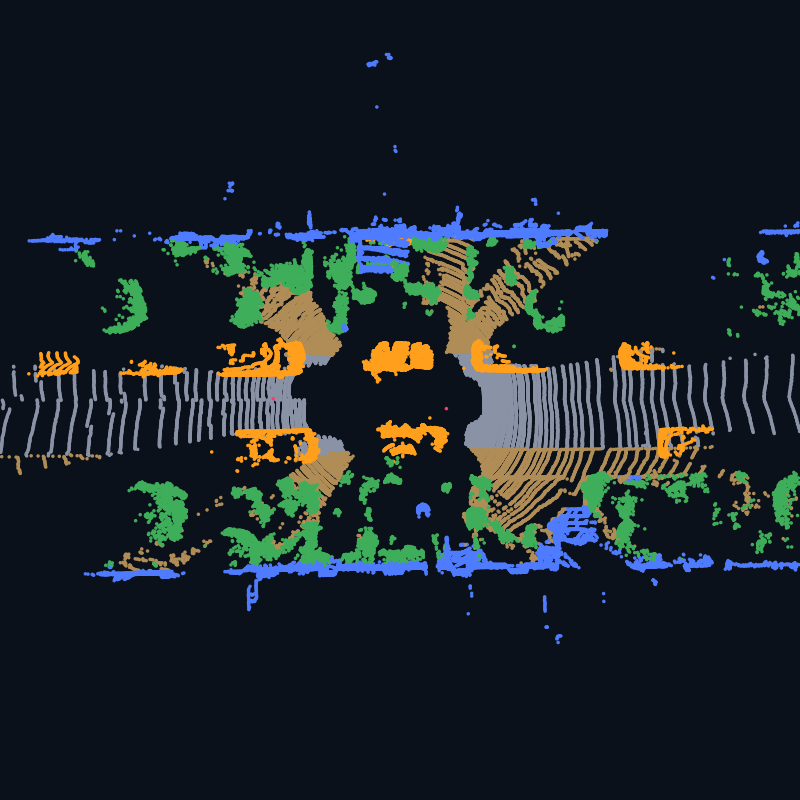
\includegraphics[width=9cm,height=9cm]{scan_output.png}};
\end{scope}

\begin{scope}[shift={(2,-8.6,0)}, every node/.style={font=\large, anchor=west}]
\fill[fill=\ConvColor] (0,0) rectangle ++(0.6,0.6); \node at (0.8,0.3) {residual block: 2 submanifold sparse convs 3$^3$ + BN + ReLU};
\fill[fill=\PoolColor, opacity=0.6] (0,-1) rectangle ++(0.6,0.6); \node at (0.8,-0.7) {stride-2 sparse conv ($\downarrow$2)};
\fill[fill=\UnpoolColor, opacity=0.6] (0,-2) rectangle ++(0.6,0.6); \node at (0.8,-1.7) {inverse sparse conv ($\uparrow$2)};
\fill[fill={rgb:white,1;black,3}, opacity=0.35] (19,0) rectangle ++(0.6,0.6); \node at (19.8,0.3) {concatenated skip features};
\fill[fill=\SoftmaxColor] (19,-1) rectangle ++(0.6,0.6); \node at (19.8,-0.7) {linear 96 $\rightarrow$ 19 classes + softmax};
\draw[copyconnection] (19,-1.7) -- ++(0.6,0); \node at (19.8,-1.7) {skip connection};
\end{scope}
\node[font=\Large\bfseries, anchor=west] at (-6,9.2,0) {Sparse 3D U-Net (FOVEA final model): 10 cm voxels, 23\,M parameters, 67.7\,\% mIoU on SemanticKITTI seq.\ 08};
\node[font=\large, anchor=west] at (-6,8.2,0) {stem 5$^3$ sparse conv $\cdot$ 4 encoder and 4 decoder stages $\cdot$ box height = voxel size (10 cm to 1.6 m), box width = channels};

\end{tikzpicture}
\end{document}
